\documentclass{article}
\usepackage[spanish]{babel}
\usepackage{lipsum}
\usepackage{natbib}
\usepackage{graphicx}
\usepackage{analysis_orax}
\usepackage{blindtext}
\usepackage{amsmath}
\usepackage{hyperref}
\usepackage{subcaption} 
\usepackage{float}
\usepackage{listings}
\usepackage{pxfonts}
\usepackage{svg}
\usepackage{pgfplots}
\pgfplotsset{compat=1.11}
\usepackage{enumitem}
\usepackage{tikz}
\usetikzlibrary{shadows}

\newcommand*{\MyShadow}{\tikz \draw [baseline, fill=blue,draw=blue,circular drop shadow] circle (2pt);}
\newcommand*{\MyBall}{\tikz \draw [baseline, ball color=red, draw=red] circle (2pt);}
\usepackage[utf8]{inputenc}

% Default fixed font does not support bold face
\DeclareFixedFont{\ttb}{T1}{txtt}{bx}{n}{8} % for bold
\DeclareFixedFont{\ttm}{T1}{txtt}{m}{n}{8}  % for normal

\definecolor{mGreen}{rgb}{0,0.6,0}
\definecolor{mGray}{rgb}{0.5,0.5,0.5}
\definecolor{mPurple}{rgb}{0.58,0,0.82}
\definecolor{backgroundColour}{rgb}{0.95,0.95,0.92}

% Custom colors
\definecolor{deepblue}{rgb}{0,0,0.5}
\definecolor{deepred}{rgb}{0.6,0,0}
\definecolor{deepgreen}{rgb}{4,0.5,0}


% Python style for highlighting
\newcommand\pythonstyle{\lstset{
language=Python,
basicstyle=\ttm,
otherkeywords={self},             % Add keywords here
keywordstyle=\ttb\color{deepblue},
commentstyle=\color{mPurple},
emph={MyClass,__init__},          % Custom highlighting
emphstyle=\ttb\color{deepred},    % Custom highlighting style
stringstyle=\color{deepgreen},
frame=tb,                         % Any extra options here
showstringspaces=false            % 
}}


% Python environment
\lstnewenvironment{python}[1][]
{
\pythonstyle
\lstset{#1}
}
{}

% Python for external files
\newcommand\pythonexternal[2][]{{
\pythonstyle
\lstinputlisting[#1]{#2}}}

% Python for inline
\newcommand\pythoninline[1]{{\pythonstyle\lstinline!#1!}}

\lstdefinestyle{CStyle}{
    backgroundcolor=\color{white},
    commentstyle=\color{mGreen},
    keywordstyle=\color{magenta},
    numberstyle=\tiny\color{mGray},
    stringstyle=\color{mPurple},
    basicstyle=\footnotesize,
    breakatwhitespace=false,         
    breaklines=true,                 
    captionpos=b,                    
    keepspaces=true,                 
    numbers=left,                    
    numbersep=5pt,                  
    showspaces=false,                
    showstringspaces=false,
    showtabs=false,                  
    tabsize=2,
    language=C
}

\title{\bigskip \bigskip \bigskip \bigskip \vspace{-15mm}\fontsize{35pt}{35pt}\selectfont\textbf{{Trabajo práctico Nº IV - FreeRTOS\\}}
\bigskip \bigskip \fontsize{18pt}{10pt}\selectfont\textbf{\textcolor{teal}{CÁTEDRA DE SISTEMAS OPERATIVOS II}}\bigskip\bigskip \bigskip\bigskip \bigskip}\bigskip\bigskip \bigskip\bigskip \bigskip % Article title
\author{
\large
{
\textsc{Casabella Martin, 39694763 }}\\[2mm]
  martin.casabella@alumnos.unc.edu.ar\\[2mm]
%\thanks{A thank you or further information}\\ % Your name
%\normalsize \href{mailto:marco.torres.810@gmail.com}{marco.torres.810@gmail.com}\\[2mm] % Your email address
\bigskip\bigskip \bigskip \bigskip\bigskip \bigskip
}

\date{\Huge\today}

%------------------Document----------------------------

\begin{document}
\maketitle
\clearpage

%-------------------------TitlePage------------------------
%\begin{titlepage}
%\end{titlepage}
%----------------------------------------------------------------------------------------
%       TITLE SECTION
%----------------------------------------------------------------------------------------

\renewcommand{\figurename}{\textbf{\textcolor{Orange}{Figura}}}
\renewcommand\thefigure{\textbf{\textcolor{Orange}{\arabic{figure}}}}

%-------------------------Content------------------------
\tableofcontents

\clearpage


\section{Introducción}
Toda aplicación de ingeniería que posea requerimientos rigurosos de tiempo, y
que este controlado por un sistema de computación, utiliza un Sistema Operativo
de Tiempo Real (RTOS, por sus siglas en ingles). \\

Una de las características principales de este tipo de SO, es su capacidad de poseer un kernel preemptive y un scheduler altamente congurable. Numerosas aplicaciones utilizan este tipo de sistemas tales como  radares, satélites, etc. lo que genera un gran
interés del mercado por ingenieros especializados en esta área.\\

\subsubsection{Objetivo}
El objetivo del presente trabajo practico es que el estudiante sea capaz de
disenar, crear, comprobar y validar una aplicación de tiempo real sobre un
RTOS.\\

\section{RTOS: conceptos principales}
Un RTOS (Real Time Operating System) es un programa que se encarga
de:
\begin{itemize}
\item Ordenar con precisión el tiempo de ejecución de las tareas
\item Administrar los recursos del sistema como tiempo de uso de
\item procesador, memoria, etc. 
\item Proveer una base consistente para el desarrollo del código
\end{itemize}

\fbox{\begin{minipage}{32em}
El RTOS crea la ilusión de múltiples tareas ejecutándose en simultáneo.
\end{minipage}}\\

El RTOS se situa entre la capa BSP (Board Support Package, o "port") y la capa de aplicación. Puede incluir varios módulos
(protocolos de red, sistema de archivos, etc.):\\

\begin{figure}[H]
   \centering
   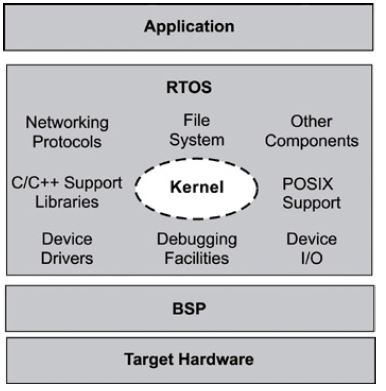
\includegraphics[width=0.4\textwidth]{figures/rtos.jpg}
   \centering
   \caption{\textbf{\textcolor{Orange}{RTOS en el sistema}}}
\end{figure}
\clearpage

Los componentes de un RTOS pueden clasificarse ampliamente en 3 grupos:
\begin{itemize}[label=$\star$]
\item \textbf{Scheduler:} maneja los hilos de ejecución de las tareas.
\item \textbf{Objetos:} tareas, colas, semáforos, etc.
\item \textbf{Servicios:} operaciones realizadas sobre los objetos (manejo de interrupciones, de memoria, etc.)
\end{itemize}

\begin{figure}[H]
   \centering
   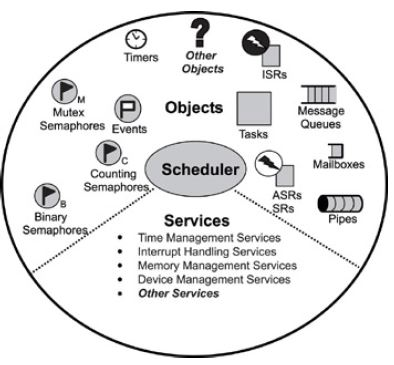
\includegraphics[width=0.6\textwidth]{figures/rtos2.jpg}
   \centering
   \caption{\textbf{\textcolor{Orange}{Componentes de un RTOS}}}
\end{figure}

\subsection{Scheduler}
El Scheduler determina cuando se ejecutar cada tarea. Existen diferentes esquemas de scheduling:\\
\begin{itemize}
\item \textbf{\textcolor{red}{Cooperativo:}} La tarea en ejecución cede el uso de CPU a otra voluntariamente.
\item \textbf{\textcolor{blue}{Preemptive:}} La tarea en ejecución cede el uso de CPU a otra por orden del scheduler.
\begin{itemize}
\item{\textcolor{blue}{Priority-Based:} Se asignan prioridades a las tareas para acceder al uso de CPU.
\begin{figure}[H]
   \centering
   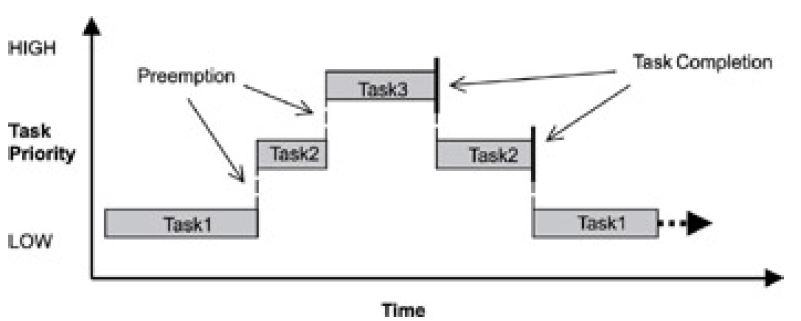
\includegraphics[width=0.6\textwidth]{figures/sch1.jpg}
   \centering
   \caption{\textbf{\textcolor{Orange}{Ejemplo de esquema Priority Based}}}
\end{figure}
}

\item{\textcolor{blue}{Round-Robin:} Se asigna un tiempo jo de uso de CPU a cada tarea en orden circular. Puede combinarse con el uso de prioridades.
\begin{figure}[H]
   \centering
   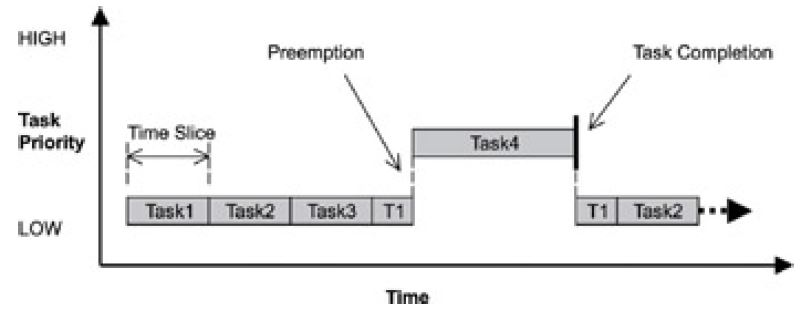
\includegraphics[width=0.6\textwidth]{figures/sch2.jpg}
   \centering
   \caption{\textbf{\textcolor{Orange}{Ejemplo de esquema Round Robin con prioridades}}}
\end{figure}
}
\end{itemize}
\end{itemize}


\subsection{Tareas}
Una tarea es un hilo de ejecución independiente que puede competir con otras tareas por tiempo de ejecución. Pueden ser creadas y eliminadas en tiempo de ejecución.\\

Se componen por:
\begin{itemize}
\item Nombre/ID
\item Prioridad (esquema preemptive)
\item Stack
\item Rutina (código)
\item Bloque de control
\end{itemize}
\begin{figure}[H]
   \centering
   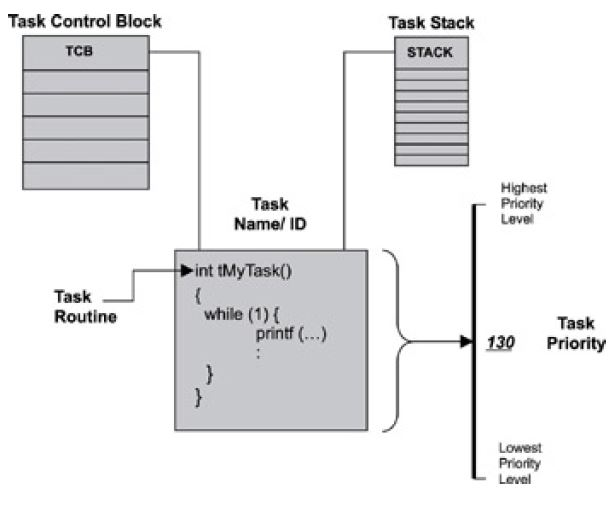
\includegraphics[width=0.5\textwidth]{figures/task1.jpg}
   \centering
   \caption{\textbf{\textcolor{Orange}{Componentes de una tarea o task}}}
\end{figure}

\clearpage

Los estados posibles de una tarea
son:
\begin{enumerate}
\item Ready: compite por tiempo de ejecución
\item Running: tarea activa 
\item Blocked: esperando pasar a Ready (podra activarse ante un evento o cuando pase cierto tiempo)
\end{enumerate}


\begin{figure}[H]
   \centering
   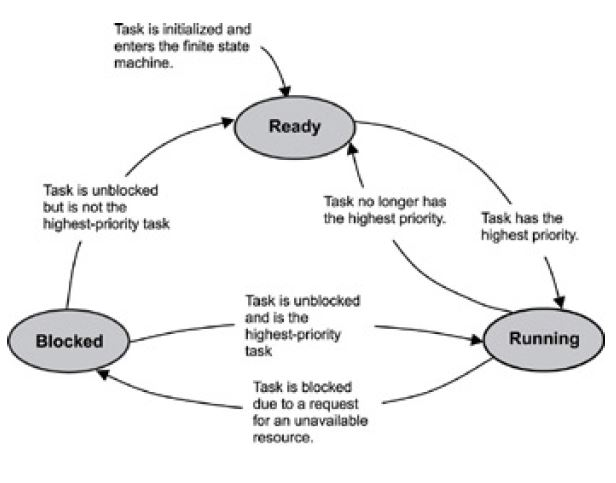
\includegraphics[width=0.57\textwidth]{figures/task2.jpg}
   \centering
   \caption{\textbf{\textcolor{Orange}{Estados posibles de una tarea}}}
\end{figure}

\subsection{Colas}
Su función principal es proveer un mecanismo de intercambio de datos entre tareas. Son FIFO.\\
Se componen por: Nombre/ID, tamaño y tipo de datos a almacenar, bloque de control. \\

\begin{figure}[H]
   \centering
   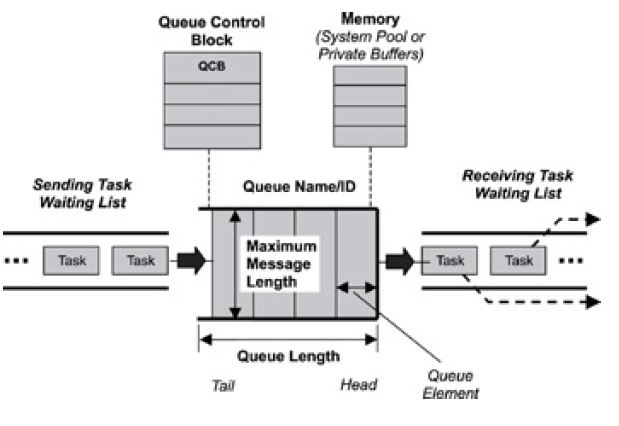
\includegraphics[width=0.6\textwidth]{figures/queue1.jpg}
   \centering
   \caption{\textbf{\textcolor{Orange}{Colas y sus componentes}}}
\end{figure}

\clearpage
\begin{itemize}
\item Varias tareas pueden acceder a una misma cola.
\item Una tarea puede elegir bloquearse si su cola esta vaca. Al llegar un elemento, automáticamente pasa a Ready.
\item Cargar datos en una cola causa una copia de los datos en memoria.
\end{itemize}

\section{FreeRTOS}

Porque el uso de FreeRTOS:\\
\begin{itemize}
\item Es de código abierto
\item Código ampliamente comentado 
\item Sencillo de portar (existen mas de 23 ports)
\item Ocupa poco espacio en  ash (5KB) necesita poca RAM (5KB + Heap) y el overhead que introduce es mínimo (entre 1\% y 4\% del tiempo de CPU) a cambio de una gran utilidad).
\item Ampliamente documentado
\item  Existe una comunidad de usuarios importante 
\item Libre de regalas. Puede ser usado en aplicaciones comerciales bajo licencia GNU versión 2.
\end{itemize}

\subsection{FreeRTOS y sistemas embebidos}
FreeRTOS es un kernel de tiempo real sobre el cual se pueden construir aplicaciones destinadas a sistemas embebidos para cumplir con sus requisitos en tiempo real.\\

Permite que las aplicaciones se organicen como una colección de hilos de ejecución independientes. Como la mayoría de los microcontroladores (como por ejemplo, Cortex-M3) tienen un solo núcleo, en realidad solo un hilo puede ejecutarse a la vez.\\

El kernel decide qué hilo se debe ejecutar al examinar la prioridad asignada a cada hilo por el diseñador de la aplicación. En el caso más simple, el diseñador de la aplicación podría asignar mayores prioridades a hilos que implementan requisitos \textit{hard real-time}l, y menores prioridades a hilos que implementan requisitos  \textit{soft real-time}. \\

Esto aseguraría que los hilos \textit{hard real-time} siempre se ejecuten por sobre los hilos \textit{soft real-time}, pero las decisiones de asignación de prioridad no siempre son tan simplistas.\\

Se detallan conceptos introducidos previamente, que serán utilizados en el trabajo.
\subsection{Tasks y freeRTOS}
Las tasks se implementan como funciones en C. La única característica especial recae en su prototitpo, que debe devolver y tomar como argumento un $void \; \; pointer$. \\

Cada tarea es un programa pequeño en si, que tiene un punto de entrada y normalmente corre en un loop infinito, y no termina. \\

Las tareas en FreeRTOS no deben tener permitido retornar de sus funciones que las implementan (i.e, no debe haber un $return$. Si no se necesita mas cierta tarea, se debe eliminar explícitamente.\\

Una única definición de la función que implementa una tarea puede crear cualquier numero de tareas desde la misma, y cada tarea sera una instancia separada de ejecución con su propia pila y su propia copia (automática) al stack de las
variables definidas para la tarea que las creo. \\

\fbox{\begin{minipage}{45em}
\textit{Si el microcontrolador corriendo la aplicación contiene un solo core, entonces una tarea puede estar en ejecución en cierto instante de tiempo. Esto implica que los estados de la misma son dos: Running y Not Running. Los demas estados, son subestados de cada uno de estos dos estados principales.}
\end{minipage}}\\

\begin{figure}[H]
   \centering
   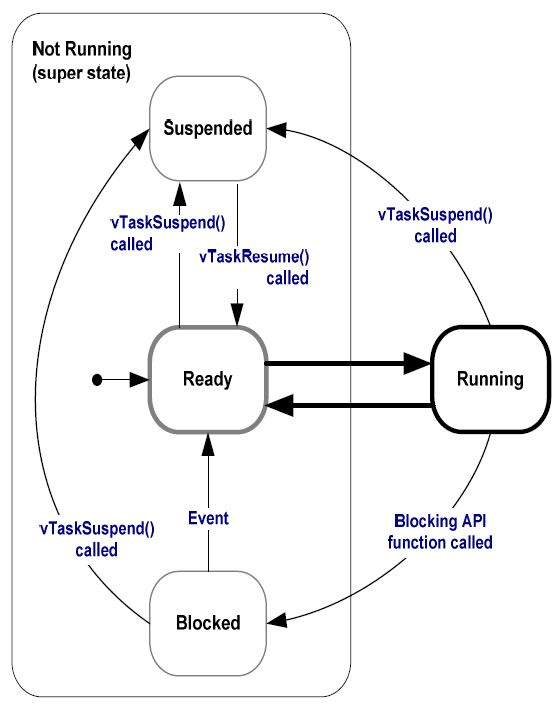
\includegraphics[width=0.6\textwidth]{figures/state.jpg}
   \centering
   \caption{\textbf{\textcolor{Orange}{Maquina de estados completa de las tareas}}}
\end{figure}




\begin{itemize}
\item Cuando una task esta en \textit{Running} el procesador esta ejecutando su codigo
\item Cuando la task esta en \textit{Not Running}, permanece inactiva, y su estado fue guardado para que pueda retomar la ejecución la próxima vez que el scheduler lo decida
\end{itemize}

Una tarea que paso de no ejecutando a en ejecución, se le dice cambiada o \textit{switched} (hay herramientas de Profiling miden estos cambios).\\

\clearpage

\subsubsection{IDLE task}
El procesador siempre necesita algo para ejecutar, y por ende, debe haber al menos una tarea en estado \textit{Running}. Para asegurar esto, se crea automáticamente por el scheduler una \textit{IDLE task}. \\

Esta tarea no hace mucho mas que estar en un loop, y se le asigna la prioridad mas baja, para evitar que no permita a una tarea de mayor prioridad, ejecutarse, y para que también ni bien una tarea de mayor prioridad pase al estado \textit{Ready}, se realice
inmediatamente la transición de estados. \\

\subsection{Queues y freeRTOS}

Las aplicaciones que utilizan FreeRTOS están estructuradas como un conjunto de tareas independientes: cada tarea es efectivamente un mini programa por derecho propio.\\

Es probable que estas tareas autónomas tengan que comunicarse entre sí para que, de forma colectiva, puedan proporcionar una funcionalidad útil del sistema. \\

La cola es la primitiva subyacente utilizada por todos mecanismos de comunicación y sincronización freeRTOS.\\

\begin{figure}[H]
   \centering
   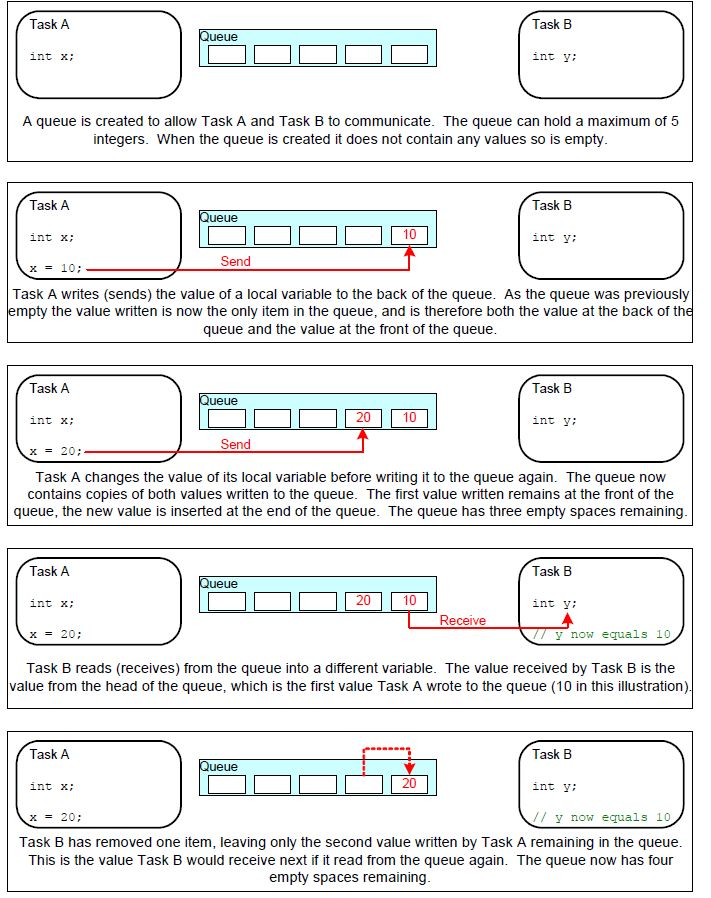
\includegraphics[width=0.65\textwidth]{figures/queue.jpg}
   \centering
   \caption{\textbf{\textcolor{Orange}{Ejemplo de secuencia de lectura y escrituras}}}
\end{figure}

\begin{itemize}
\item Una cola puede tener un numero finito de elementos de tamano fijo
\item El tamano y la longitud de la cola se establecen cuando la misma es creada
\item Las colas se utilizan como buffers FIFO, en donde los datos escritos van al final de la cola (tail), y se remueven desde el frente (head). No obstante, se puede modificar
\item Escribir datos en la cola causa una copia byte a byte. Leer de la cola, implica otra copia byte a byte.
\end{itemize}


\textbf{LECTURA Y BLOQUEO}\\

Cuando una tarea intenta leer de una cola, puede adicionalmente setear su tiempo de bloqueo. Esto se define como el tiempo que la tarea debe permanecer bloqueada
esperando que haya datos disponibles en la cola para leer (i.e, trata de leer y la cola se haya vacía).\\

Una tarea bloqueada por este motivo, automáticamente pasa a estar lista (\textit{Ready}) cuando otra tarea o alguna interrupción, coloca datos en la cola involucrada. Lo mismo ocurre si expira el tiempo seteado, automáticamente cambia su estado a \textit{Ready}.Siempre se desbloqueara primero aquella de mayor prioridad, y de tener todas la misma prioridad, se despertara a aquella que mas tiempo haya estado esperando. \\


\textbf{ESCRITURA Y BLOQUEO}\\

También se puede setear el tiempo (máximo en este caso) que una tarea se bloquea cuando no puede escribir en la cola involucrada. Esto ocurriria si la cola se encuentra llena en el momento que la tarea apunta a escribir un dato. \\

Al tener muchos escritores, puede ocurrir que mas de una tarea se bloquee, lo que recae en que solo una se desbloqueara cuando haya espacio. Tal como ocurre con la lectura, el criterio de desbloqueo es el mismo. \\

\subsubsection{Acceso a colas por múltiples tareas}

Las colas son objetos que existen por si mismo, y no tienen tarea propietaria ni están asignadas a ninguna en particular.\\

Cualquier numero de tareas puede escribir y leer en la misma cola. De hecho, una cola con múltiples escritores es una necesidad común.\\

\section{Setup del sistema}

El sistema consta por un lado, en el embebido LPC1769 , donde se encuentra instalado FreeRTOS, que ejecuta la aplicacion de tiempo real. Por otro lado, la placa se encuentra conectada a la PC, desde donde se observan diferentes métricas Tracealyzer. \\

El proyecto se ejecutara en una computadora con Windows como sistema operativo residennte. Existe conectividad entre el embebido y la PC mediante UART. Se utilizo el integrado CP2102 como controlador USB para conectar la placa a la PC. \\

La PC tiene instalado el software LPCXpresso v8.2.2, y el software Tracealyzer 4 en su versión de prueba. La versión de FreeRTOS instalada, es la v10.0.1.\\

Se instalo ademas, un plugin para Eclipse (LPCXpresso esta basado en eclipse) para Tracealyzer 4, que permite que el software de profiling lea los datos rastreados utilizando la interfaz de \textit{debug} normal, permitiendo que cualquier dispositivo y \textit{Debug probe} que el IDE soporte emplee este plugin. \\

\begin{figure}[H]
   \centering
   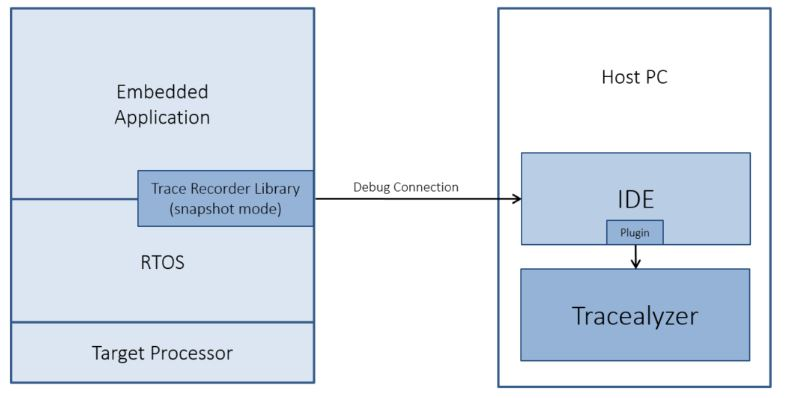
\includegraphics[width=0.7\textwidth]{figures/plugin.jpg}
   \centering
   \caption{\textbf{\textcolor{Orange}{Debug y tracealyzer con el plugin instalado}}}
\end{figure}


\section{Programa con dos tareas simples}

Se utilizo un ejemplo de los anexados en la bibliografia utilizada, que consiste de dos tareas simples, y una cola. Una de las tareas es la emisora de mensajes, mientras que otra
es la receptora. \\

Este programa se utilizo para familiarizarse con Tracealyzer y sus funcionalidades. \\

Vemos en primera instancia, la interacción en el tiempo entre las tareas y demás eventos intermedios:\\
\begin{figure}[H]
   \centering
   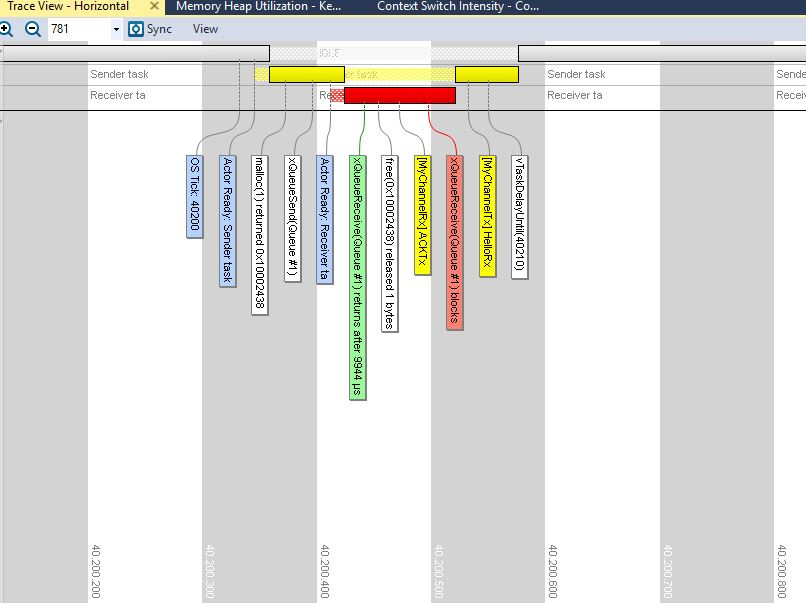
\includegraphics[width=0.7\textwidth]{figures/trace1.jpg}
   \centering
   \caption{\textbf{\textcolor{Orange}{Seccion de la traza capturada}}}
\end{figure}

En cuanto al flujo de comunicación, vemos los actores involucrados junto con los objetos que utilizan:\\
\begin{figure}[H]
   \centering
   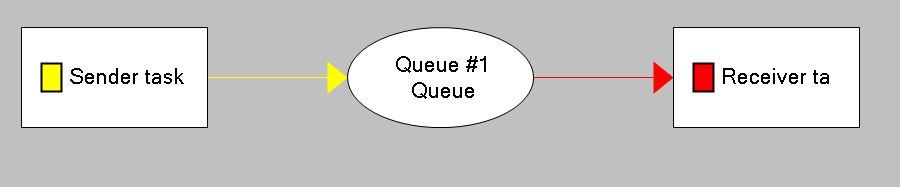
\includegraphics[width=0.9\textwidth]{figures/trace6.jpg}
   \centering
   \caption{\textbf{\textcolor{Orange}{Flujo de comunicación}}}
\end{figure}

\bigskip
\bigskip
\bigskip
\bigskip
\bigskip
\bigskip
\bigskip



Podemos también analizar el cambio de contexto en la aplicación corriendo:\\
\begin{figure}[H]
   \centering
   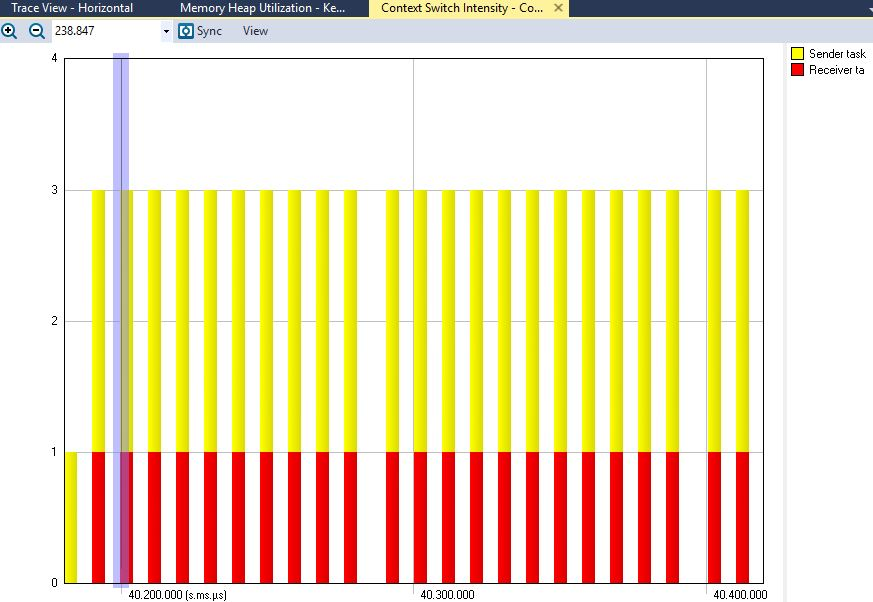
\includegraphics[width=0.8\textwidth]{figures/trace2.jpg}
   \centering
   \caption{\textbf{\textcolor{Orange}{Context switching}}}
\end{figure}

\begin{figure}[H]
   \centering
   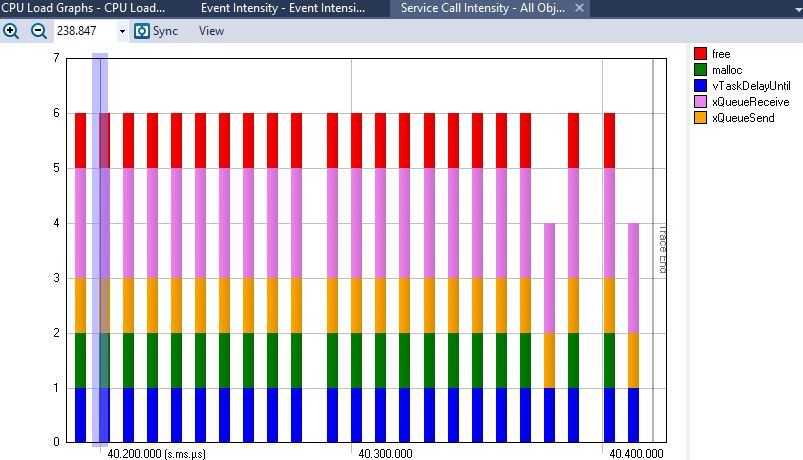
\includegraphics[width=0.9\textwidth]{figures/trace3.jpg}
   \centering
   \caption{\textbf{\textcolor{Orange}{Carga CPU}}}
\end{figure}

\begin{figure}[H]
   \centering
   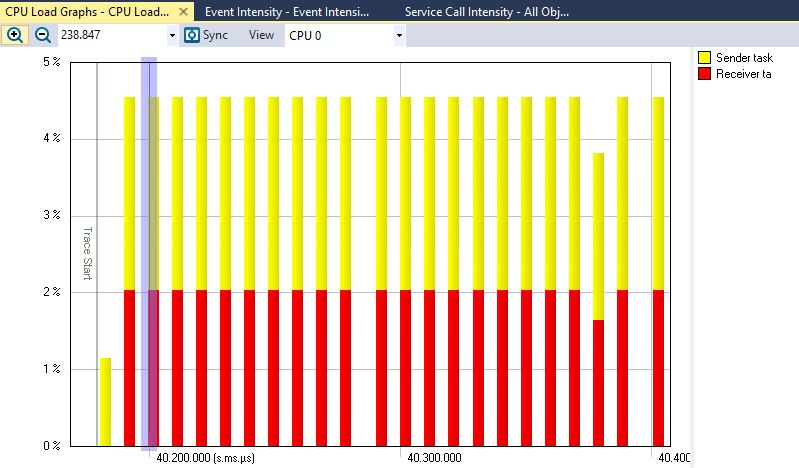
\includegraphics[width=0.8\textwidth]{figures/trace4.jpg}
   \centering
   \caption{\textbf{\textcolor{Orange}{Intensidad de llamados a servicios}}}
\end{figure}

Vemos que en este caso tenemos unicamente una cola (objeto), y podemos ver la utilización de la misma por parte de las tareas corriendo:\\
\begin{figure}[H]
   \centering
   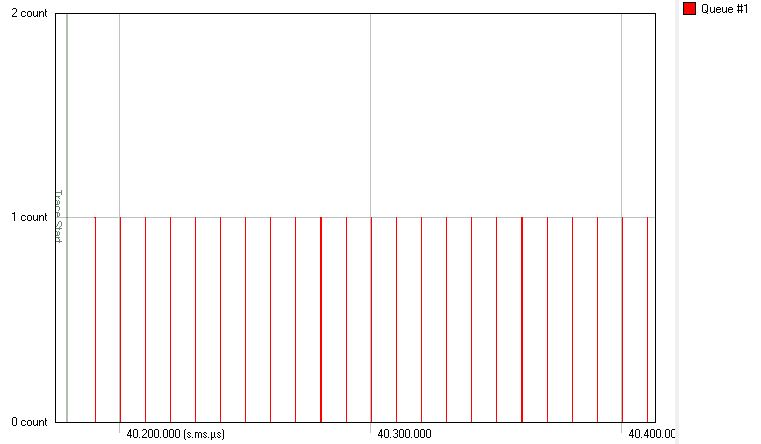
\includegraphics[width=0.8\textwidth]{figures/trace5.jpg}
   \centering
   \caption{\textbf{\textcolor{Orange}{Utilización de objetos}}}
\end{figure}

\begin{figure}[H]
   \centering
   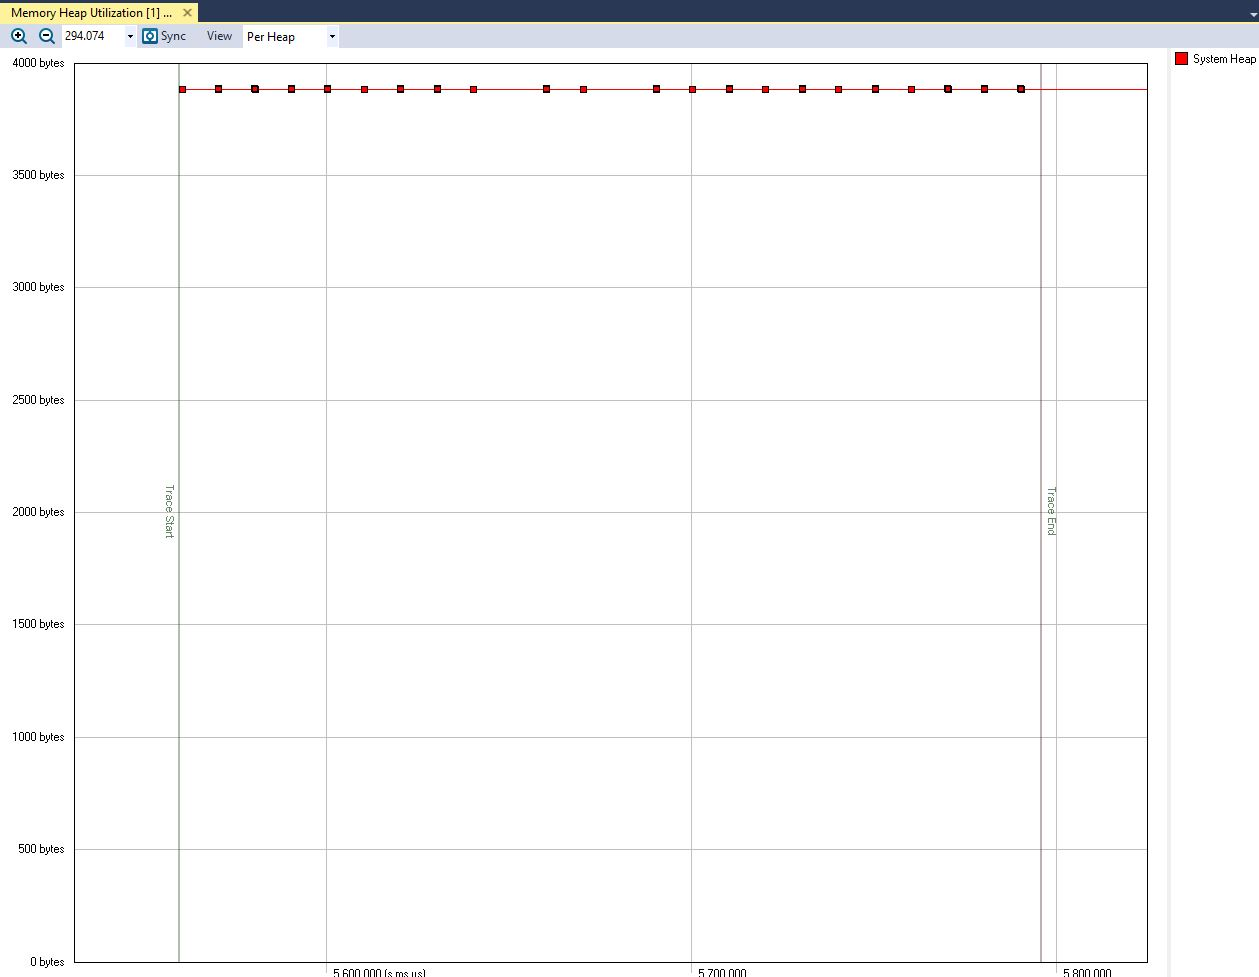
\includegraphics[width=0.8\textwidth]{figures/trace7.jpg}
   \centering
   \caption{\textbf{\textcolor{Orange}{Memory Heap}}}
\end{figure}


\begin{figure}[H]
   \centering
   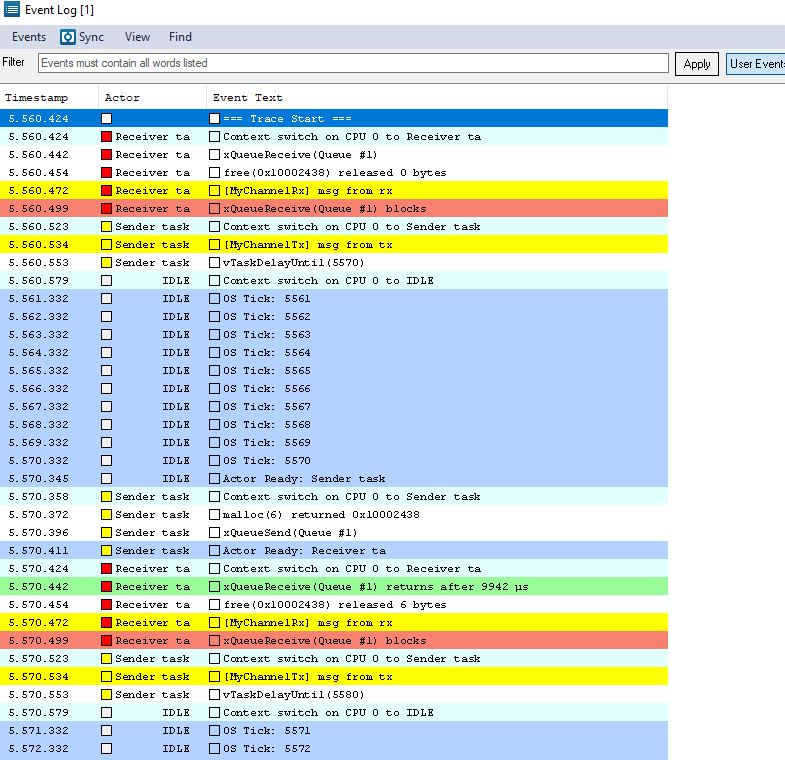
\includegraphics[width=0.8\textwidth]{figures/trace8.jpg}
   \centering
   \caption{\textbf{\textcolor{Orange}{Event log}}}
\end{figure}


\subsection{Código}
\begin{lstlisting}[style=CStyle]

#ifdef __USE_CMSIS
#include "LPC17xx.h"
#endif

#include <cr_section_macros.h>
#include <stdlib.h>
/* Kernel includes. */
#include "FreeRTOS.h"
#include "task.h"
#include "queue.h"

/* Priorities at which the tasks are created. */
#define mainQUEUE_RECEIVE_TASK_PRIORITY		( tskIDLE_PRIORITY + 2 )

#define	mainQUEUE_SEND_TASK_PRIORITY		( tskIDLE_PRIORITY + 1 )

/* The bit of port 0 that the LPCXpresso LPC13xx LED is connected. */
#define mainLED_BIT 						( 22 )

/* The rate at which data is sent to the queue, specified in milliseconds. */
#define mainQUEUE_SEND_FREQUENCY_MS			( 10 / portTICK_RATE_MS )

/* The number of items the queue can hold.  This is 1 as the receive task
will remove items as they are added, meaning the send task should always find
the queue empty. */


#define mainQUEUE_LENGTH					( 1 )

/*
 * The tasks as described in the accompanying PDF application note.
 */
 
static void prvQueueReceiveTask( void *pvParameters );
static void prvQueueSendTask( void *pvParameters );
void vConfigureTimerForRunTimeStats( void );

/*
 * Simple function to toggle the LED on the LPCXpresso LPC17xx board.
 */
 
static void prvToggleLED( void );

/* The queue used by both tasks. */
static xQueueHandle xQueue = NULL;



int main(void)
{
	/* Initialise P0_22 for the LED. */
	
	LPC_PINCON->PINSEL1	&= ( ~( 3 << 12 ) );
	LPC_GPIO0->FIODIR |= ( 1 << mainLED_BIT );

	/* Init and start tracing */
	vTraceEnable(TRC_START);

	/* Create the queue. */
	xQueue = xQueueCreate( mainQUEUE_LENGTH, sizeof(char)*4 );

	if( xQueue != NULL )
	{
		/* Start the two tasks as described in the accompanying application
		note. */
		
		xTaskCreate( prvQueueReceiveTask, ( signed char * ) "Rx", configMINIMAL_STACK_SIZE, NULL, mainQUEUE_RECEIVE_TASK_PRIORITY, NULL );
		xTaskCreate( prvQueueSendTask, ( signed char * ) "TX", configMINIMAL_STACK_SIZE, NULL, mainQUEUE_SEND_TASK_PRIORITY, NULL );

		/* Start the tasks running. */
		vTaskStartScheduler();
	}

	/* If all is well we will never reach here as the scheduler will now be
	running.  If we do reach here then it is likely that there was insufficient
	heap available for the idle task to be created. */
	
	for( ;; );
}



static void prvQueueSendTask( void *pvParameters )
{
	portTickType xNextWakeTime;
	
	char* log;
	
	/* Initialise xNextWakeTime - this only needs to be done once. */
	
	xNextWakeTime = xTaskGetTickCount();
	
	/*The first step to visualizing custom information that is specific to your application is to create a user event
	 *  channel. This is basically a string output channel that allows a developer to add their own custom events, called
	 *   User events in Tracealyzer. 
	 *   
	 *   For example, if I wanted to transmit sensor event data, I would first create the channel using the following
	 *    code:  traceString MyChannel = xTraceRegisterString(“DataChannel”);
	 *    
	 *    In case your compiler does not recognize this function, you need to #include “trcRecorder.h”
	 *    
	 *    This function registers a user event channel named DataChannel in the trace. This makes Tracealyzer 
	 *    show a checkbox for this channel in the filter panel, so you can easily enable/disable the display of
	 *     these events. */

	traceString ch = xTraceRegisterString("MyChannelTx");

	for( ;; )
	{
		/* Place this task in the blocked state until it is time to run again.
		The block state is specified in ticks, the constant used converts ticks
		to ms.  While in the blocked state this task will not consume any CPU
		time. */

		vTracePrint(ch, "msg from tx");
		vTaskDelayUntil( &xNextWakeTime, mainQUEUE_SEND_FREQUENCY_MS );

		/* Send to the queue - causing the queue receive task to flash its LED.
		0 is used as the block time so the sending operation will not block -
		it shouldn't need to block as the queue should always be empty at this
		point in the code. */
		log = pvPortMalloc(sizeof(char)*(rand()%8));
		xQueueSend( xQueue, &log, 0 );
	}
}


static void prvQueueReceiveTask( void *pvParameters )
{
	char * log;
	traceString ch = xTraceRegisterString("MyChannelRx");

	for( ;; )
	{

		vTracePrint(ch, "msg from rx");
		
		/* Wait until something arrives in the queue - this task will block
		indefinitely provided INCLUDE_vTaskSuspend is set to 1 in
		FreeRTOSConfig.h. */
		
		xQueueReceive( xQueue, &log, portMAX_DELAY );

		/*  To get here something must have been received from the queue, but
		is it the expected value?  If it is, toggle the LED. */
		
		vPortFree(log);
		prvToggleLED();
	}
}



static void prvToggleLED( void )
{
unsigned long ulLEDState;

	/* Obtain the current P0 state. */
	ulLEDState = LPC_GPIO0->FIOPIN;

	/* Turn the LED off if it was on, and on if it was off. */
	LPC_GPIO0->FIOCLR = ulLEDState & ( 1 << mainLED_BIT );
	LPC_GPIO0->FIOSET = ( ( ~ulLEDState ) & ( 1 << mainLED_BIT ) );
	

void vConfigureTimerForRunTimeStats( void )
{
const unsigned long TCR_COUNT_RESET = 2, CTCR_CTM_TIMER = 0x00, TCR_COUNT_ENABLE = 0x01;

	/* This function configures a timer that is used as the time base when
	collecting run time statistical information - basically the percentage
	of CPU time that each task is utilising.  It is called automatically when
	the scheduler is started (assuming configGENERATE_RUN_TIME_STATS is set
	to 1). */

	/* Power up and feed the timer. */
	LPC_SC->PCONP |= 0x02UL;
	LPC_SC->PCLKSEL0 = (LPC_SC->PCLKSEL0 & (~(0x3<<2))) | (0x01 << 2);

	/* Reset Timer 0 */
	LPC_TIM0->TCR = TCR_COUNT_RESET;

	/* Just count up. */
	LPC_TIM0->CTCR = CTCR_CTM_TIMER;

	/* Prescale to a frequency that is good enough to get a decent resolution,
	but not too fast so as to overflow all the time. */
	LPC_TIM0->PR =  ( configCPU_CLOCK_HZ / 10000UL ) - 1UL;

	/* Start the counter. */
	LPC_TIM0->TCR = TCR_COUNT_ENABLE;
}
\end{lstlisting}




\clearpage
\section{Programa con dos productores y un consumidor}
Ya familiarizado con el software, se procedió a realizar la aplicación principal de este trabajo. \\

Se debe de implementar una aplicación que posea dos productores y un consumidor.\\

El primero de los productores es una tarea que genera strings de caracteres de longitud variable (ingreso de comandos por teclado). Para emular esto, se realizo una función
que genera strings de longitud aleatoria, y la misma es utilizada por la tarea aperiódica implementada. Se opto esta solucion para no agregar un periférico como es un teclado, y evitar emergentes adicionales, ya que no es el objetivo del trabajo, \\

La segunda tarea tarea, es un valor numérico de longitud fija, proveniente del sensor de temperatura del embebido. De la misma manera, se emula esta situacion enviando
un valor numérico entre 0 y 255 generado, representando las medidas. \\

El consumidor, es una tarea que envía el valor recibido a la terminal de una computadora por puerto serie (UART).


\begin{figure}[H]
   \centering
   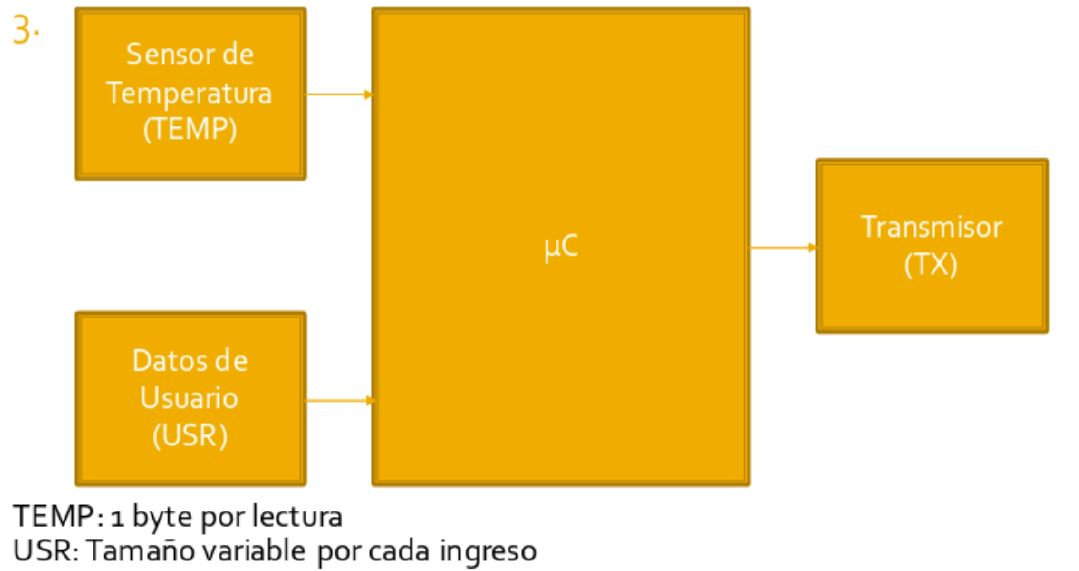
\includegraphics[width=0.8\textwidth]{figures/arq.jpg}
   \centering
   \caption{\textbf{\textcolor{Orange}{Arquitectura por componentes del sistema a implementar}}}
\end{figure}

\subsubsection{Solución al uso de una sola cola y datos de tamaño variable}
La solución a utilizar una sola cola donde ademas, sus elementos no tienen tamaño fijo, se realizo con el uso de estructuras. \\

Se utilizo una cola para transferir estructuras, donde un campo $char$ y otro campo $char \; * \; (string)$  permiten llevar a cabo la implementacion requerida. \\

La cola entonces alberga estructuras, donde de tratarse de el ingreso del usuario, el campo $msg$ tendrá contenido de longitud variable, mientras que el campo $num$ no se considera. De tratarse de un dato proveniente del sensor, el campo $msg$ ahora torna a ser un $NULL$ $pointer$, y no se considera, permitiendo identificar las diferentes fuentes (o
tareas) que escriben en la cola. \\

\begin{lstlisting}[style=CStyle]
		struct msg_struct {
				char * msg;
				char num;
				int len_str;
		};
\end{lstlisting}


Luego declaramos una cola de punteros a estructura, y la creamos:\\

\begin{lstlisting}[style=CStyle]
			#define MAX_POINTERS		10
			
			/* Declare a variable of type QueueHandle_t to hold the handle of the queue being created. */
			QueueHandle_t xPointerQueue
			
			/* Create a queue that can hold a maximum of MAX_POINTERS pointers*/
			xPointerQueue = xQueueCreate(MAX_POINTERS, sizeof(struct msg_struct *)); 
\end{lstlisting}

\subsection{Debug en entorno Semihosted - versión intermedia}
Semihosting es un mecanismo que permite que el código que se ejecuta en un destino ARM se comunique y use las facilidades de entrada / salida en una computadora host que ejecuta un depurador.\\

Ejemplos de estas funciones incluyen entrada de teclado, salida de pantalla y E / S de disco. Por ejemplo, puede utilizar este mecanismo para habilitar funciones en la biblioteca de C, como $printf()$ y $scanf()$, para usar la pantalla y el teclado del host en lugar de tener una pantalla y teclado en el sistema de destino.\\


Se creo un proyecto \textit{semihost}, para primero poder ver la correcta emulación tanto del sensor, como del ingreso del usuario (teclado). Vemos que ambas
tareas emulan correctamente al sensor y a la entrada variable:\\
\begin{figure}[H]
   \centering
   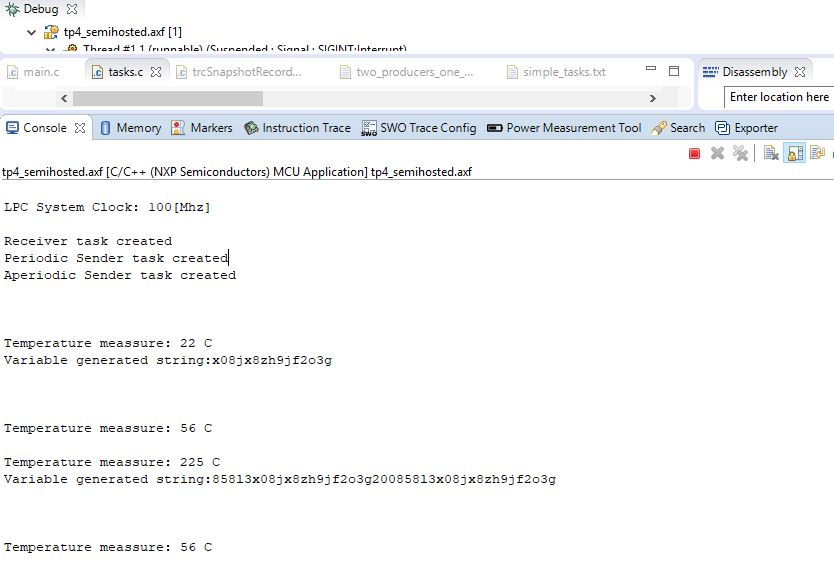
\includegraphics[width=0.87\textwidth]{figures/semihost.jpg}
   \centering
   \caption{\textbf{\textcolor{Orange}{Prueba de tareas productoras en entorno semihost}}}
\end{figure}

En cuanto a la versión final, se utilizo el mismo código a excepción de una función adicional para que la tarea consumidora pueda enviar los datos via UART. \\

En esta versión (semihsoted), en lugar de proceder a enviar cada dato que se lee, simplemente se imprimen por pantalla, por ende, la tarea consumidora solo lee y muestra resultados por pantalla.\\

\subsection{Versión final}

La versión final ya consta de la aplicación receptora interactuando con la PC mediante el envio de los datos leidos a traves del puerto serie. \\

\textbf{Prioridades:}
Si se configura que la tarea consumidora sea la de mayor prioridad, y las dos tareas productoras tengan la misma, la cola nunca tendrá mas que 1 ítem (estructura) en ella. \\

Esto es causado porque la tarea consumidora se antepone (\textit{pre-empting}) a las tareas productoras ni bien se coloca un dato en la cola.\\
\begin{figure}[H]
   \centering
   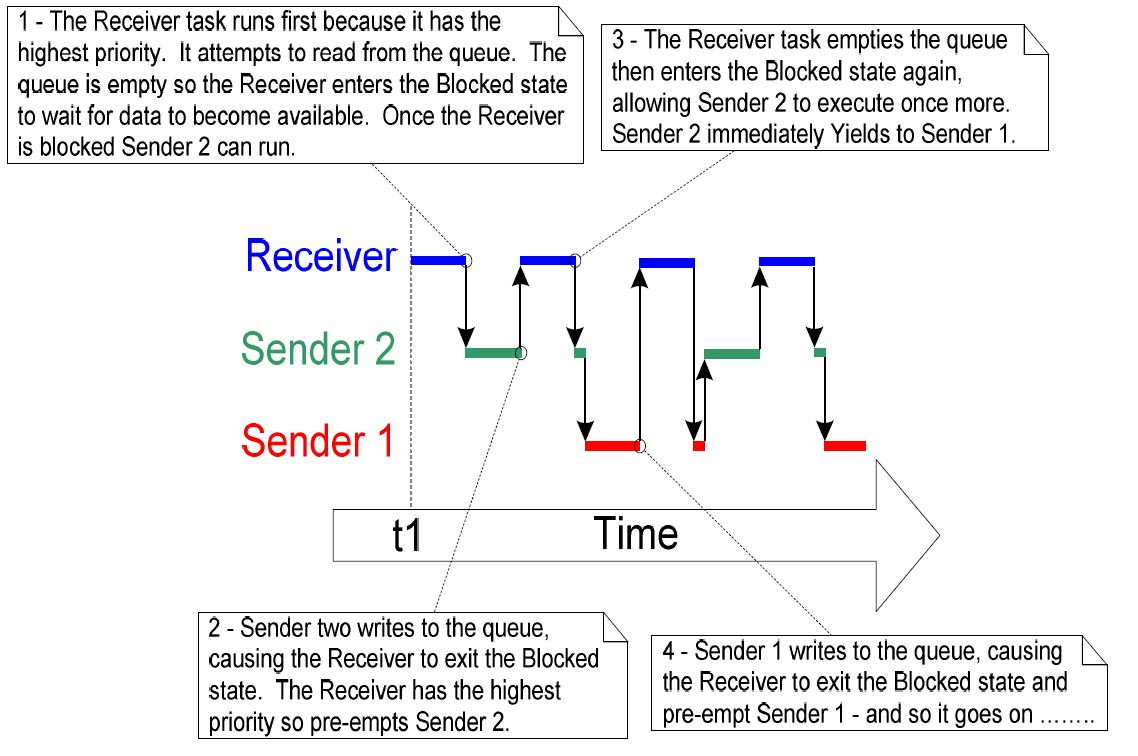
\includegraphics[width=0.8\textwidth]{figures/pri2.jpg}
   \centering
   \caption{\textbf{\textcolor{Orange}{Secuencia de ejecución con tarea consumidora de mayor prioridadd}}}
\end{figure}
 

Por otro lado, si las tareas productoras son las de mayor prioridad, la cola estará normalmente llena. \\

Esto se debe a que ni bien la tarea consumidora saque un ítem de la cola, se le antepone alguna de las dos tareas productoras que luego vuelve a llenar la cola. \\
\clearpage

La tarea productora vuelve a bloquearse para asi esperar que se libere espacio y volver a disponer de la cola nuevamente.\\
\begin{figure}[H]
   \centering
   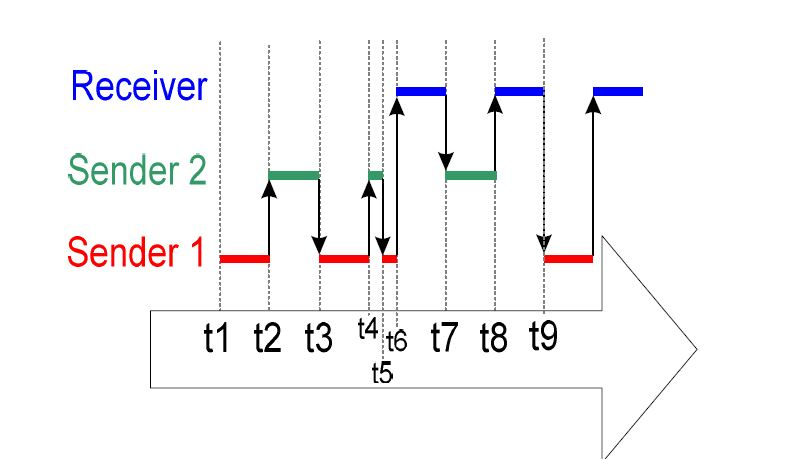
\includegraphics[width=0.6\textwidth]{figures/pri1.jpg}
   \centering
   \caption{\textbf{\textcolor{Orange}{Secuencia de ejecución con tareas productoras de mayor prioridad}}}
\end{figure}
 
 Se configuro de menor prioridad a la tarea consumidora, mientras que las tareas productoras tienen ambas la misma prioridad. Se procede a mostrar su funcionamiento y luego se agregan los códigos empleados junto con el análisis vía Tracealyzer.\\
 
 
Se tiene un script en Python que configura el puerto con los parámetros necesarios, y se encarga de recibir los datos que la tarea consumidora (Tx en el diagrama en bloques de la arquitectura anexado) envía (hacer zoom a captura en caso que no se vea nitidamente):
\begin{figure}[H]
   \centering
   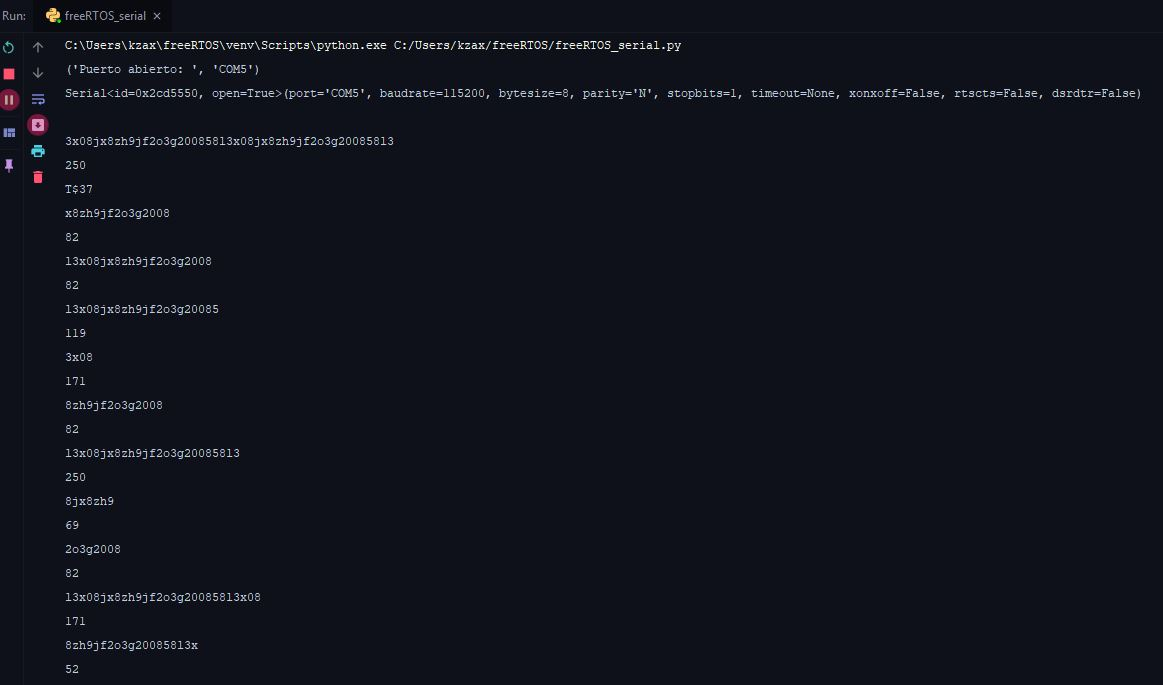
\includegraphics[width=1.0\textwidth]{figures/serial.jpg}
   \centering
   \caption{\textbf{\textcolor{Orange}{Recepción de datos vía Pyserial}}}
\end{figure}


\subsubsection{Análisis con Tracealyzer}

\begin{figure}[H]
   \centering
   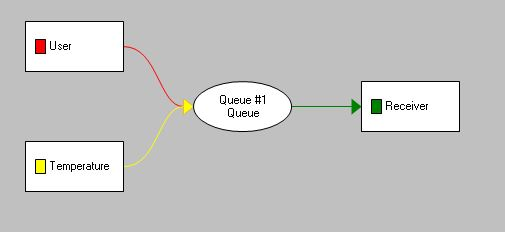
\includegraphics[width=0.8\textwidth]{figures/trace9.jpg}
   \centering
   \caption{\textbf{\textcolor{Orange}{Actores y objetos involucrados}}}
\end{figure}

\begin{figure}[H]
   \centering
   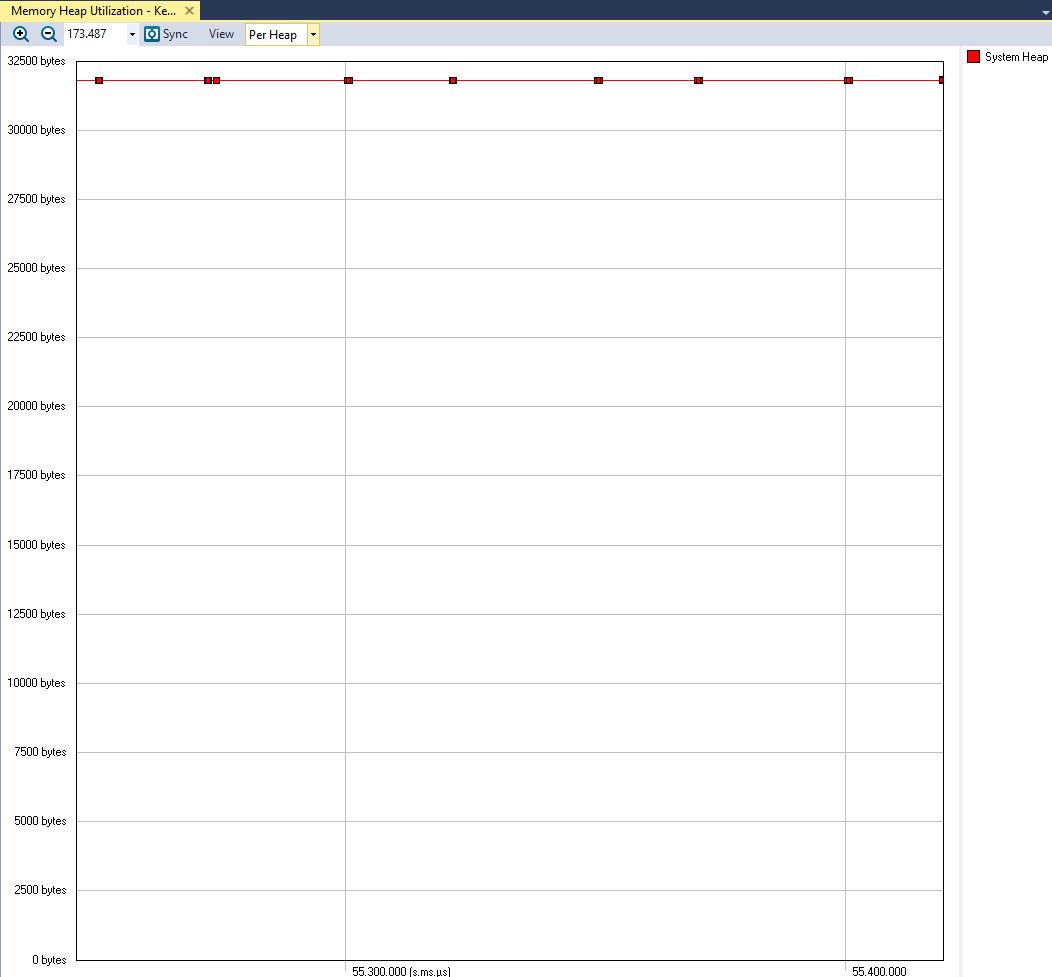
\includegraphics[width=0.8\textwidth]{figures/trace10.jpg}
   \centering
   \caption{\textbf{\textcolor{Orange}{Memory heap}}}
\end{figure}

\begin{figure}[H]
   \centering
   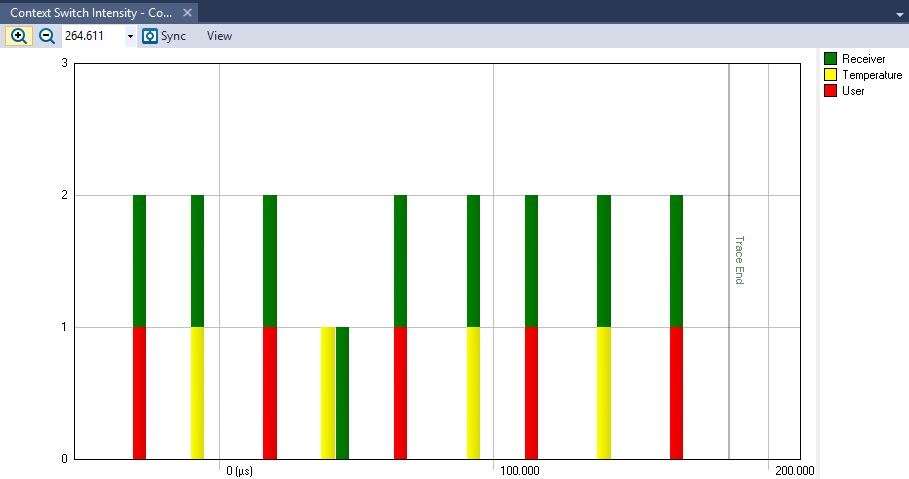
\includegraphics[width=0.8\textwidth]{figures/trace11.jpg}
   \centering
   \caption{\textbf{\textcolor{Orange}{Context switching}}}
\end{figure}

\begin{figure}[H]
   \centering
   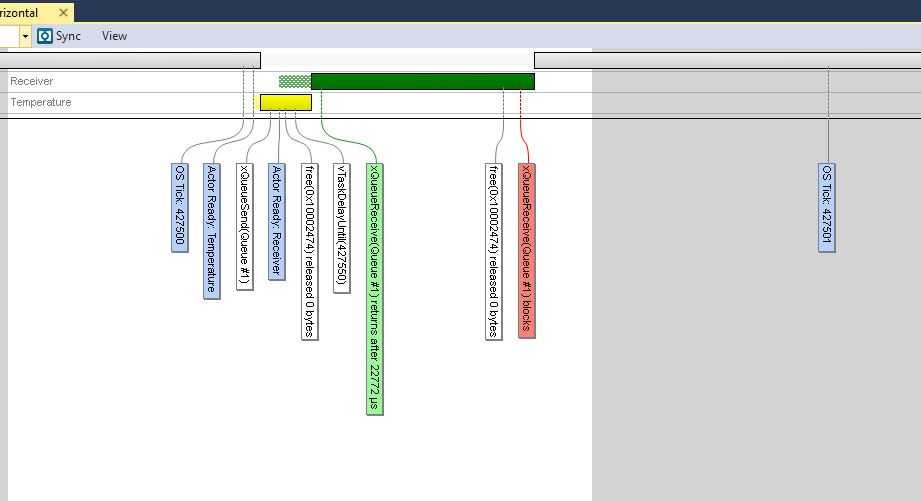
\includegraphics[width=0.8\textwidth]{figures/trace13.jpg}
   \centering
   \caption{\textbf{\textcolor{Orange}{Secuencia temperature - receiver}}}
\end{figure}

\begin{figure}[H]
   \centering
   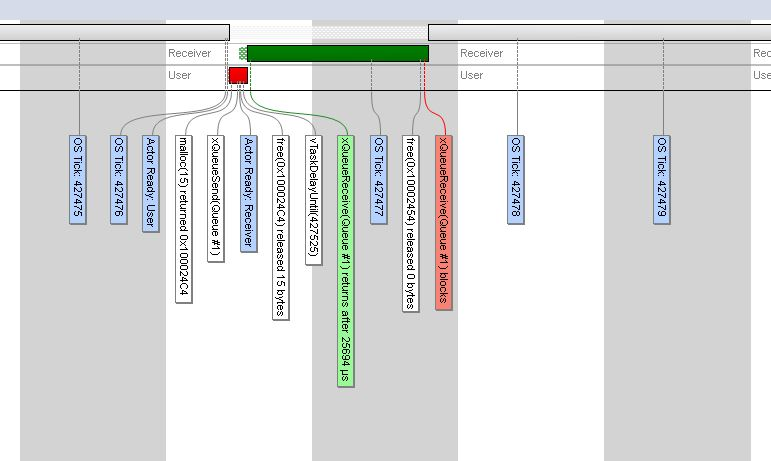
\includegraphics[width=0.9\textwidth]{figures/trace14.jpg}
   \centering
   \caption{\textbf{\textcolor{Orange}{Secuencia user - receiver}}}
\end{figure}
\begin{figure}[H]
   \centering
   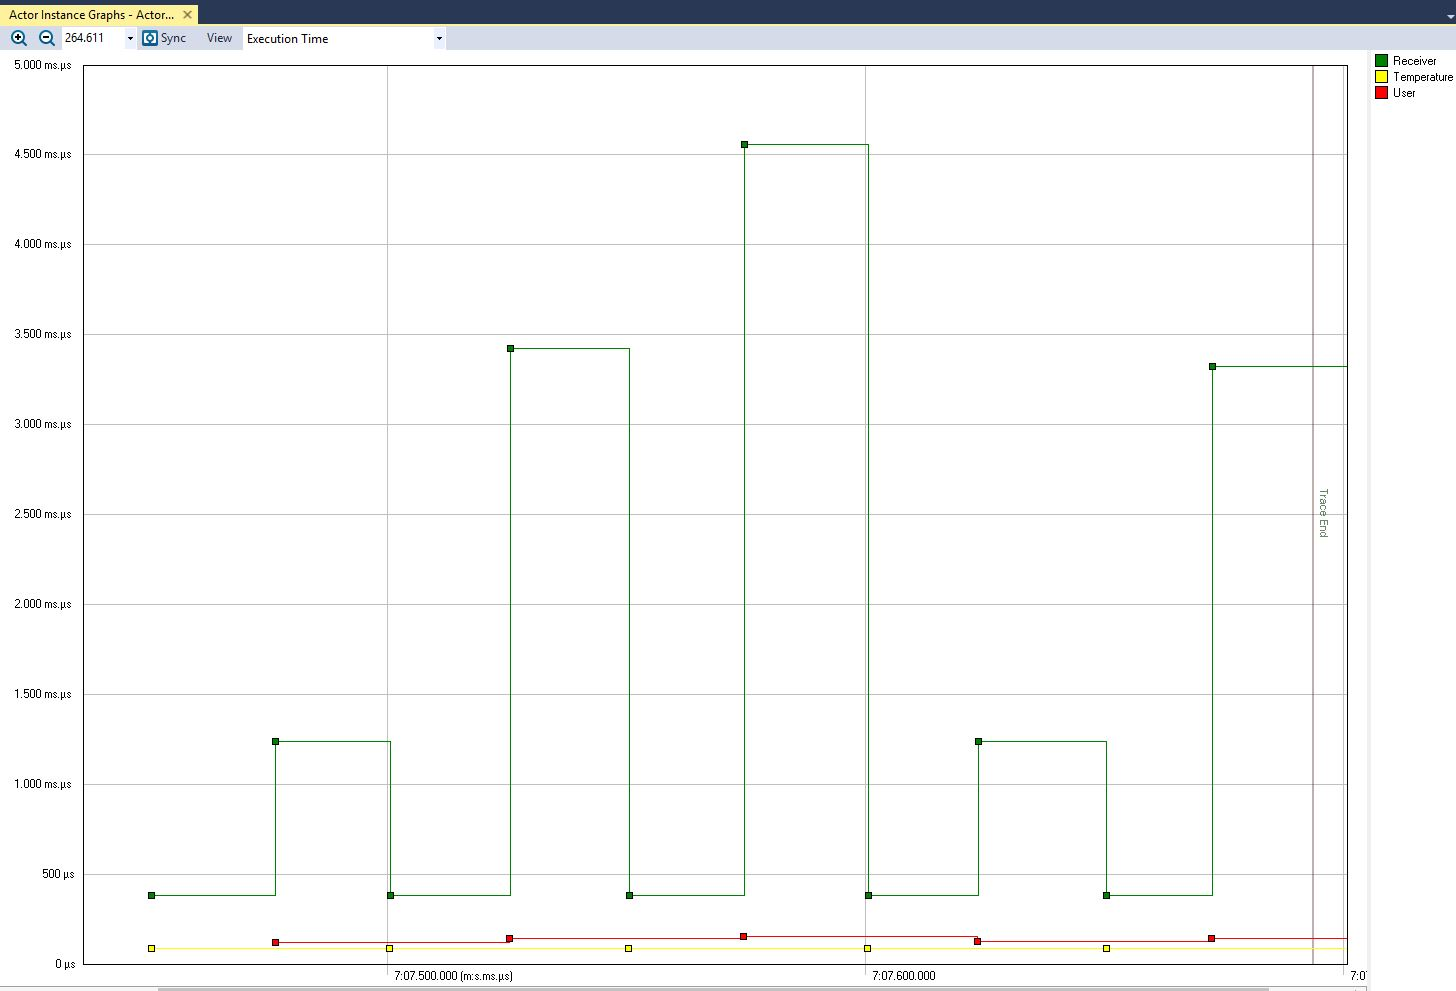
\includegraphics[width=1.0\textwidth]{figures/trace12.jpg}
   \centering
   \caption{\textbf{\textcolor{Orange}{Tiempo de ejecución de cada actor}}}
\end{figure}



\begin{figure}[H]
   \centering
   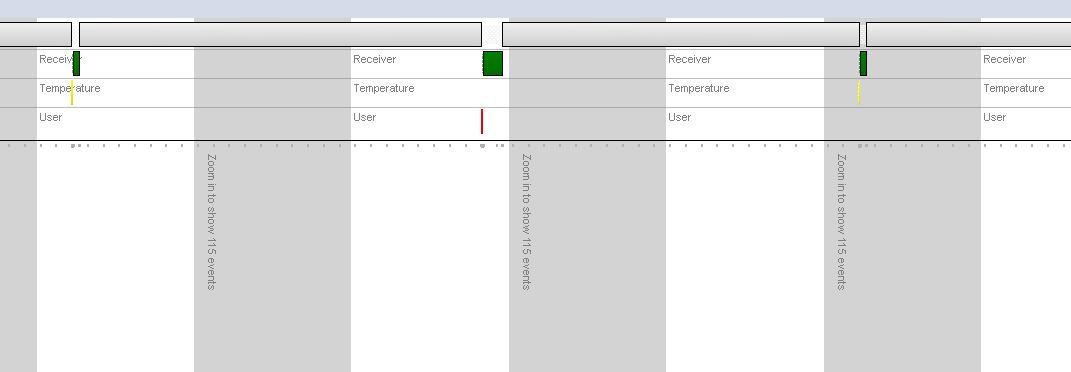
\includegraphics[width=1.0\textwidth]{figures/trace15.jpg}
   \centering
   \caption{\textbf{\textcolor{Orange}{Interleaving}}}
\end{figure}


\begin{figure}[H]
   \centering
   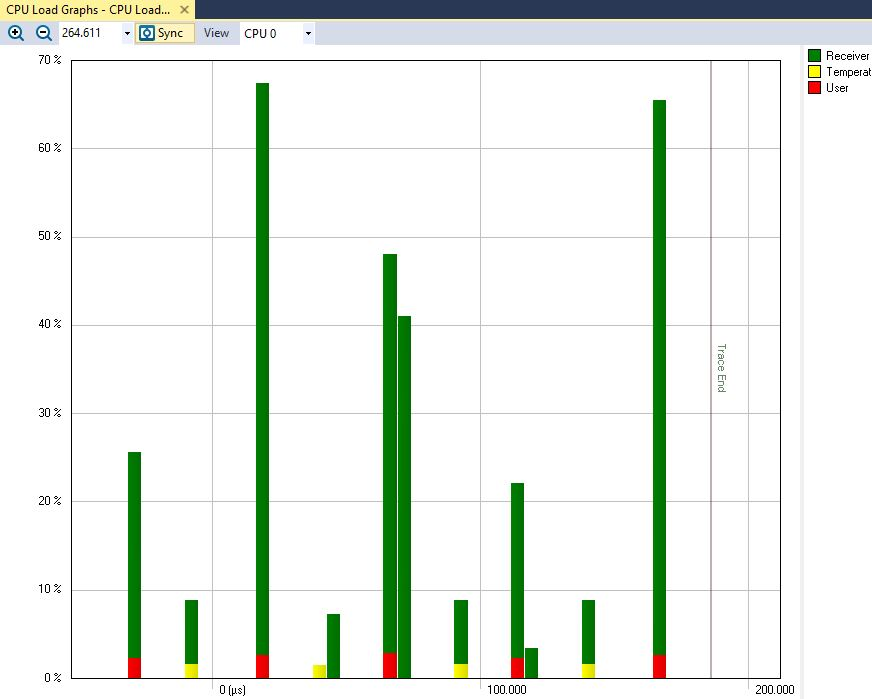
\includegraphics[width=1.0\textwidth]{figures/trace16.jpg}
   \centering
   \caption{\textbf{\textcolor{Orange}{Grafo de carga del CPU}}}
\end{figure}


\begin{figure}[H]
   \centering
   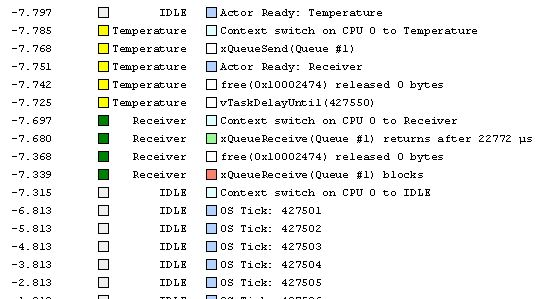
\includegraphics[width=1.0\textwidth]{figures/trace17.jpg}
   \centering
   \caption{\textbf{\textcolor{Orange}{Event log - secuencia Temperature - Receiver}}}
\end{figure}


\begin{figure}[H]
   \centering
   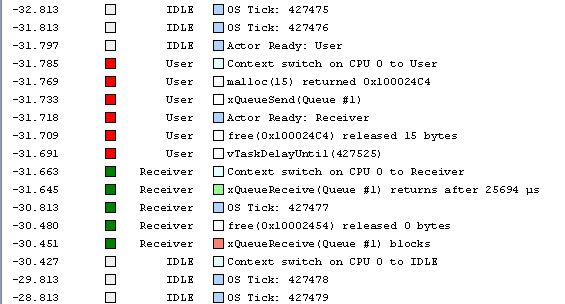
\includegraphics[width=1.0\textwidth]{figures/trace18.jpg}
   \centering
   \caption{\textbf{\textcolor{Orange}{Event log - secuencia User - Receiver}}}
\end{figure}

\clearpage


\subsubsection{Código}
\begin{lstlisting}[style=CStyle]
/*
 * TP4 OSII - FreeRTOS
 *
 * @author Casabella Martin *
 *
 *
 * */

#include <string.h>
#include <math.h>
/* Kernel includes. */
#include "FreeRTOS.h"
#include "task.h"
#include "queue.h"
#include <stdio.h>
#include <stdlib.h>
#include <string.h>

/* Priorities at which the tasks are created. */
#define RECEIVE_TASK_PRIORITY		( tskIDLE_PRIORITY + 1 )
#define	PERIODIC_TASK_PRIORITY		( tskIDLE_PRIORITY + 4 )
#define	APERIODIC_TASK_PRIORITY		( tskIDLE_PRIORITY + 4 )
/* The bit of port 0 that the LPCXpresso LPC13xx LED is connected. */
#define mainLED_BIT 						( 22 )
#define MAX_POINTERS		10

/* The rate at which data is sent to the queue, specified in milliseconds. */
#define PERIODIC_SEND_FREQUENCY_MS			( 50 / portTICK_RATE_MS )

#define MAX_STRING_LEN	51

#define BUF_TEMP 10
#define portNEW_DELAY 200

/*Prototipos de funciones*/
static void vReceiverTask(void *pvParameters);
static void vPeriodicSenderTask(void *pvParameters);
static void vAperiodicSenderTask(void *pvParameters);

static void vToggleLED(void);
char * vRandomString(int len_string);

void UART3_Init(void);
void UART_Send(char* datos, int size);

/* Declare a variable of type QueueHandle_t to hold the handle of the queue being created. */
QueueHandle_t xPointerQueue;

/*Estructura para uso de strings variables*/
struct msg_struct {
	char * msg;
	char num;
	int len_str;
};

int main(void) {
	/* P0_22 for the LED. */
	LPC_PINCON->PINSEL1 &= (~(3 << 12));
	LPC_GPIO0->FIODIR |= (1 << mainLED_BIT);

	/* Enable traceanalycer snapshot */
	vTraceEnable(TRC_START);

	/* Create a queue that can hold a maximum of MAX_POINTERS pointers*/
	xPointerQueue = xQueueCreate(MAX_POINTERS, sizeof(struct msg_struct *)); //creo cola de 10 punteros a struct

	if (xPointerQueue != NULL) {

		/*
		 * The size of the stack used by the idle task is defined by the applicationdefined constant configMINIMAL_STACK_SIZE . The value assigned to
		 * this constant in the standard FreeRTOS Cortex-M3 demo applications is the minimum recommended for any task. If your task uses a lot of stack
		 * space, then you must assign a larger value.		 *
		 *
		 *For example, the Cortex-M3 stack is 32 bits wide so, if
		 *usStackDepth is passed in as 100, then 400 bytes of stack space will be allocated (100 * 4 bytes).
		 *
		 */

		//taskcode, name, stacksize, parameters, handletask
		xTaskCreate(vReceiverTask, "Receiver", configMINIMAL_STACK_SIZE,
		NULL, RECEIVE_TASK_PRIORITY, NULL);

		xTaskCreate(vPeriodicSenderTask, "TemperatureSensor",
		configMINIMAL_STACK_SIZE, NULL, PERIODIC_TASK_PRIORITY,
		NULL);

		xTaskCreate(vAperiodicSenderTask, "User", configMINIMAL_STACK_SIZE,
				NULL, APERIODIC_TASK_PRIORITY	, NULL);

		/*Dimos prioridades iguales a ambas tareas productoras, mientras que la lectora tiene prioridad mas alta*/

		/**
		 * Passing a uxPriority value above (configMAX_PRIORITIES – 1) will result in the priority assigned to the task being capped silently to the
		 * maximum legitimate value.
		 *
		 */

		vTaskStartScheduler();

	}

	/* If all is well we will never reach here as the scheduler will now be
	 running.  If we do reach here then it is likely that there was insufficient
	 heap available for the idle task to be created. */
	for (;;)
		;
	return 0;
}


/**
 * Tarea de envio periodico representando el seensor de temperatura. Se genera
 * un valor entre 0 y 255, emulando medicion, y esta tarea se encarga de comunicarla
 * con el proceso central.
 *
 *
 * @param void*  pvParameters
 */
static void vPeriodicSenderTask(void *pvParameters) {

	/*	This parameter is named on the assumption that vTaskDelayUntil() is
	 being used to implement a task that executes periodically and with a
	 fixed frequency. */

	/* The xLastWakeTime variable needs to be initialized with the current tick
	 count. Note that this is the only time the variable is written to explicitly.
	 After this xLastWakeTime is updated automatically internally within
	 vTaskDelayUntil(). */
	portTickType xLastWakeTime;
	xLastWakeTime = xTaskGetTickCount();

	/* Define a task that performs an action every 50 milliseconds. */
	const TickType_t xPeriod = pdMS_TO_TICKS(50);

	struct msg_struct *msg = pvPortMalloc(sizeof(struct msg_struct *));

	/* Enter the loop that defines the task behavior. */
	for (;;) {

		/* This task should execute every 50 milliseconds. Time is measured
		 in ticks. The pdMS_TO_TICKS macro is used to convert milliseconds
		 into ticks. xLastWakeTime is automatically updated within vTaskDelayUntil()
		 so is not explicitly updated by the task. */

		/* Place this task in the blocked state until it is time to run again.
		 The block state is specified in ticks, the constant used converts ticks
		 to ms.  While in the blocked state this task will not consume any CPU
		 time.

		 The parameters to vTaskDelayUntil() specify, instead, the exact tick count value at which the
		 calling task should be moved from the Blocked state into the Ready state. vTaskDelayUntil()
		 is the API function that should be used when a fixed execution period is required (where you
		 want your task to execute periodically with a fixed frequency), as the time at which the calling
		 task is unblocked is absolute, rather than relative to when the function was called (as is the
		 case with vTaskDelay()).

		 */
		vTaskDelayUntil(&xLastWakeTime, xPeriod);

		msg->msg = NULL;
		msg->num = (char) (rand() % 255); //genero valor aleatorio de 0 a 255 y lo casteo a char

		/* Send to the queue - causing the queue receive task to flash its LED.
		 *
		 * 	0 is used as the block time so the sending operation will not block -
		 * 	it shouldn't need to block as the queue should always be empty at this
		 * 	point in the code.
		 *
		 * 	*/

		/*(pdMS_TO_TICKS(5): The maximum amount of time the task should remain in the
		 *Blocked state to wait for space to become available on the queue,
		 *should the queue already be full.*/
		xQueueSend(xPointerQueue, &msg, pdMS_TO_TICKS(5));
		//espera 5 [ms] si la cola esta llena
		

		/*Free a estructura*/
		vPortFree(msg);

	}
}

/**
 * Funcion Aperiodica representa el ingreso de caracteres de un usuario. Se genera una cadena de longitud
 * variable, de manera aleatoria, y se envia aperiodicamente (i,e cada cierto tiempo que tambien es variable)
 *
 * @param: void*  pvParameters
 *
 */
static void vAperiodicSenderTask(void *pvParameters) {

	portTickType xLastWakeTime;
	/*Aloco estructura donde colocara cada string generado para colocar en la cola*/
	struct msg_struct *msg = pvPortMalloc(sizeof(struct msg_struct *));
	msg->msg = pvPortMalloc(sizeof(char *));
	msg->num = 0; //le asigno 0 para que no tenga mugre el campo

	int random_len = 0;

	xLastWakeTime = xTaskGetTickCount();

	/* Define a task that performs an action every random milisecons starting (at least 20)*/
	const TickType_t xPeriod = pdMS_TO_TICKS((rand() % (150 - 20) + 20));
	/*Esta tarea dura entre 20 ms y 150     rand()%(nMax-nMin) + nMin; */

	for (;;) {
		/* Place this task in the blocked state until it is time to run again.
		 The block state is specified in ticks, the constant used converts ticks
		 to ms.  While in the blocked state this task will not consume any CPU
		 time. */
		vTaskDelayUntil(&xLastWakeTime, xPeriod);

		random_len = (rand() + xTaskGetTickCount()) % (MAX_STRING_LEN - 3);

		/* Send to the queue - causing the queue receive task to flash its LED.*/
		msg->msg = vRandomString(random_len);
		msg->len_str = random_len + 2; //+2 porque no incluye el \0

		/*Envio string, esperando hasta 5[ms]  si la cola esta llena
		 *
		 * xQueueSend(), xQueueSendToFront() and xQueueSendToBack() will
		 * return immediately if xTicksToWait is zero and the queue is already full.
		 *
		 * */
		xQueueSend(xPointerQueue, &msg, pdMS_TO_TICKS(5));
		
		/*Free a estructura*/
		vPortFree(msg->msg);
	}

}

/**
 * Tarea de recepcion. Se fija en la cola si hay algo y lo recibe. Compara campos de la estructura, y lo
 * reenvia por puerto serie.
 *
 *
 * @param void*  pvParameters
 */

static void vReceiverTask(void *pvParameters) {

	struct msg_struct * pcReceivedValue; //creo puntero a estructura

	//char cReceivedValue;
	char tmp_buf[BUF_TEMP];

	/*Modulo UART*/
	UART3_Init();

	for (;;) {
		/* Wait until something arrives in the queue - this task will block
		 indefinitely provided INCLUDE_vTaskSuspend is set to 1 in
		 FreeRTOSConfig.h. */

		/* Receive the address of a buffer. */
		if (xQueueReceive(xPointerQueue, /* The handle of the queue. */
		&pcReceivedValue, /* Store the buffer’s address in pcReceivedString. */
		portNEW_DELAY) == pdTRUE) {

			if (pcReceivedValue->msg == NULL) {
				/*Vino valor de temperatura*/

				/*Convierto valor recibido, a base 10, y lo pongo en tmp buf*/
				itoa(pcReceivedValue->num, tmp_buf, 10);

				/*Concateno \r\n*/
				strcat(tmp_buf, "\r\n");

				/*Mando la temperatura recibida a traves del puerto UART*/
				UART_Send(tmp_buf, strlen(tmp_buf));

			} else {

				/*Vino string de longitud variable (msg tiene algo)*/

				/*Lo mando directamente (ya es char*, no necesito casteo)*/
				UART_Send(pcReceivedValue->msg, pcReceivedValue->len_str);

			}

			/* toggle LED 22 */
			vToggleLED();
			/*Free a estructura*/
			vPortFree(pcReceivedValue);

		}

//		} else {
//			/* Returned if data cannot be read from the queue because the queue is
//			 * already empty.
//			 *
//			 * If a block time was specified (xTicksToWait was not zero) then the
//			 * calling task will have been placed into the Blocked state to wait for
//			 * another task or interrupt to send data to the queue, but the block time
//			 * expired before this happened.
//			 *
//			 */
//		}

	}

}

/*
 * Funcion para generar string de longitud variable. No solo varia la longitud de
 * la cadena, sino que la posicion dentro del arreglo fijo, i.e, si genero una cadena
 * de largo 5, no implica que sean los primeros 5 caracteres siempre.
 *
 * @param: len_str longitud de la cadena devuelta
 * @return: char*	cadena generada
 *
 * */

char * vRandomString(int len_string) {
	static char* leters = "a0b1c2d3e4f5g6h7i8j9k0l1m2n3o4p5q6r7s8t9u0v1w2x3y4z5";

	/* +3 para el agregado de \r\n */
	char* var_string = pvPortMalloc(len_string += 3);

	for (int i = 0; i < len_string - 3; i++) {
		var_string[i] = leters[rand() % MAX_STRING_LEN]; //elige elemento con indice de 0 a 50
	}
	var_string[len_string - 3] = '\r';
	var_string[len_string - 2] = '\n';
	var_string[len_string - 1] = '\0';

	return var_string;
}

/**
 * toggle LED 22
 */
static void vToggleLED(void) {
	unsigned long ulLEDState;

	/* Obtain the current P0 state. */
	ulLEDState = LPC_GPIO0->FIOPIN;

	/* Turn the LED off if it was on, and on if it was off. */
	LPC_GPIO0->FIOCLR = ulLEDState & (1 << mainLED_BIT);
	LPC_GPIO0->FIOSET = ((~ulLEDState) & (1 << mainLED_BIT));
}

/**
 * configuracion UART
 */
void UART3_Init(void) {

	/*UART3, chau UART1*/
	LPC_SC->PCONP |= (1 << 25);
	/*Deshabilito tambien UART0 y UART1*/
	LPC_SC->PCONP &= ~(3 << 3);
	/*PCLKSEL1*/
	LPC_SC->PCLKSEL1 |= (1 << 18);

	/*Palabra de 8 bits*/
	LPC_UART3->LCR = 0x03;
	/*Bit de stop*/
	LPC_UART3->LCR |= (1 << 2);
	/*Habilito configuarcion*/
	LPC_UART3->LCR |= 0b10000000;
	LPC_UART3->DLL = 54; //*U3LCR 0b10100001 ; // 115200
	LPC_UART3->DLM = 0; //*U3LCR
	/*Deshabilito cfg baudrate*/
	LPC_UART3->LCR &= ~(1 << 7);

	//pin 0 TXD0 pin 1 RXD0 puerto 0
	LPC_PINCON->PINSEL0 = 0b1010; // *PINSEL0 configurar los pines port 0
	LPC_PINCON->PINMODE0 = 0; // *PINMODE0 pin a pull up

	/*
	 * LPC_UART3->IER = 1; // *U3IER habilito la interrupcion por Recive Data Aviable
	 * *ISER0 |= 1<<8; //activate interrup uart3
	 */
}

void UART_Send(char* data, int size) {
	for (int i = 0; i < size; i++) {
		while ((LPC_UART3->LSR & (1 << 5)) == 0) {
		} //*U3LSR // Wait for Previous transmission
		LPC_UART3->THR = data[i]; //*U3THR
	}
}

void vConfigureTimerForRunTimeStats(void) {
	const unsigned long TCR_COUNT_RESET = 2, CTCR_CTM_TIMER = 0x00,
			TCR_COUNT_ENABLE = 0x01;

	/* This function configures a timer that is used as the time base when
	 collecting run time statistical information - basically the percentage
	 of CPU time that each task is utilising.  It is called automatically when
	 the scheduler is started (assuming configGENERATE_RUN_TIME_STATS is set
	 to 1). */

	/* Power up and feed the timer. */
	LPC_SC->PCONP |= 0x02UL;
	LPC_SC->PCLKSEL0 = (LPC_SC->PCLKSEL0 & (~(0x3 << 2))) | (0x01 << 2);

	/* Reset Timer 0 */
	LPC_TIM0->TCR = TCR_COUNT_RESET;

	/* Just count up. */
	LPC_TIM0->CTCR = CTCR_CTM_TIMER;

	/* Prescale to a frequency that is good enough to get a decent resolution,
	 but not too fast so as to overflow all the time. */
	LPC_TIM0->PR = ( configCPU_CLOCK_HZ / 10000UL) - 1UL;

	/* Start the counter. */
	LPC_TIM0->TCR = TCR_COUNT_ENABLE;
}

/*
 * Necessary functions for FreeRTOS
 */
void vApplicationStackOverflowHook(TaskHandle_t pxTask, char *pcTaskName) {
	/* This function will get called if a task overflows its stack. */
	(void) pxTask;
	(void) pcTaskName;
	for (;;)
		;
}

\end{lstlisting}
\subsubsection{Script Python para comunicación serial}
\pythonexternal{freeRTOS_serial.py}

\clearpage
\nocite{*}   % all not cited bib entrys are shown in bibliography ...
\bibliographystyle{unsrt} % <===========================================
\bibliography{biblio}

%\begin{figure}[H]
   %\centering
   %\includegraphics[width=0.6\textwidth]{figures/timestamp2.jpg}
   %\centering
   %\caption{\textbf{\textcolor{Orange}{Otro ejemplo de operación del algoritmo de sellado de tiempo}}}
%\end{figure}





 
%\begin{figure}[H]
    %\centering
      %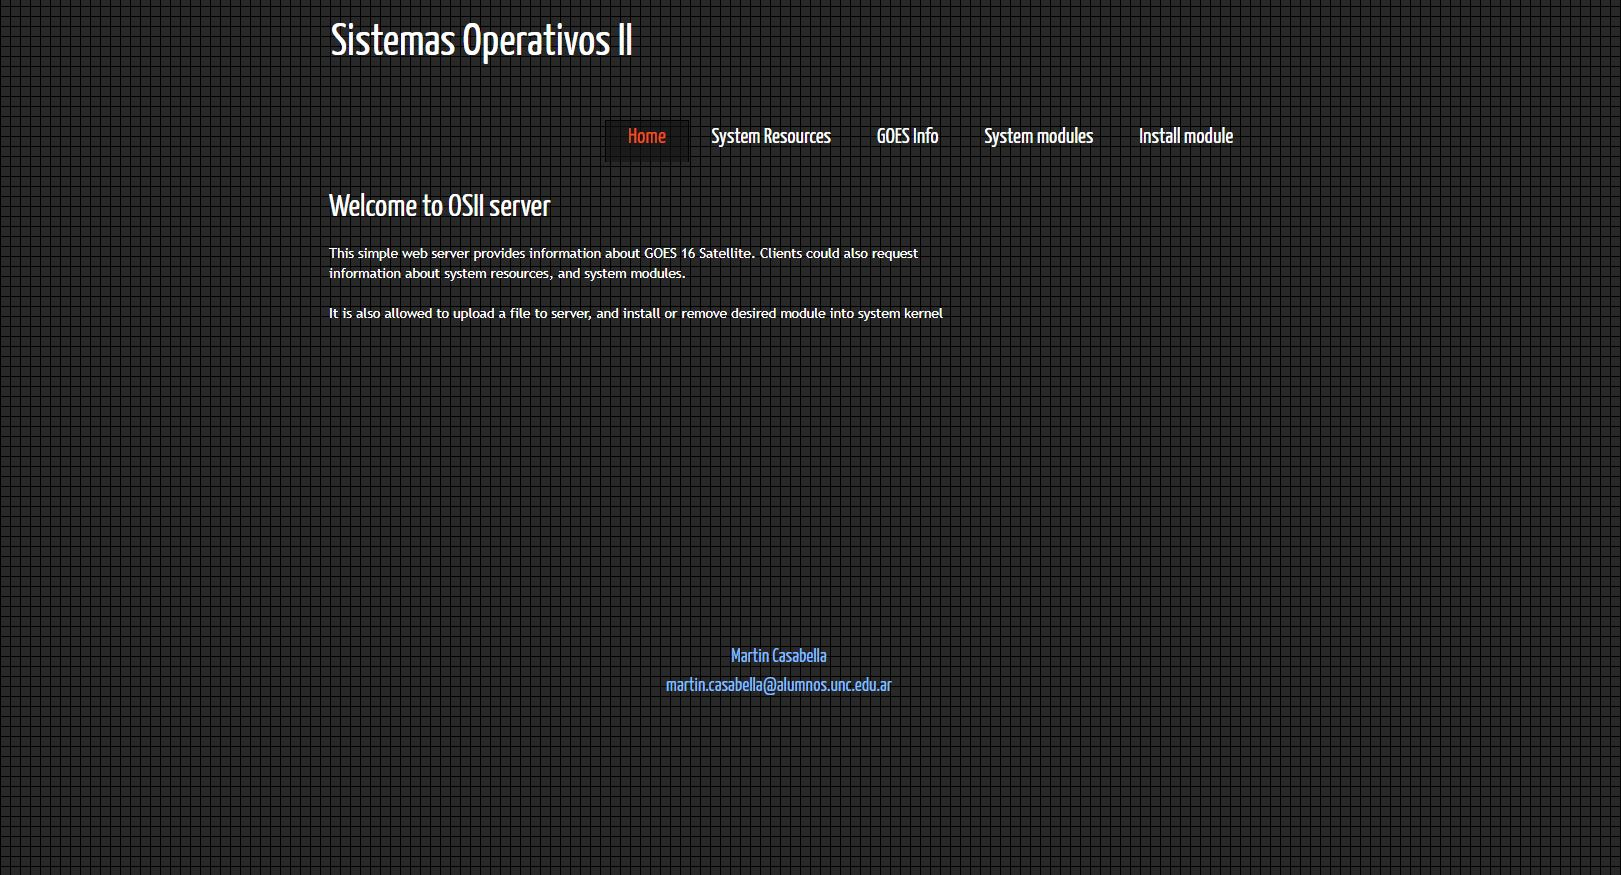
\includegraphics[width=0.8\textwidth]{figures/1.jpg}
       %\centering
       %\caption{\textbf{\textcolor{Orange}{Pagina principal}}}
    %\end{figure}




\end{document}